\section{Results}

\subsection{High level design}
The heart of our system is a Convolution Module(CM).  This module is dedicated to performing convolution on input images.  It uses a dedicated cache, as well as a new instruction that allows the compiler to take advantage of a massively parallel, specialized convolution pipeline to speed up the convolution process.

\begin{center}
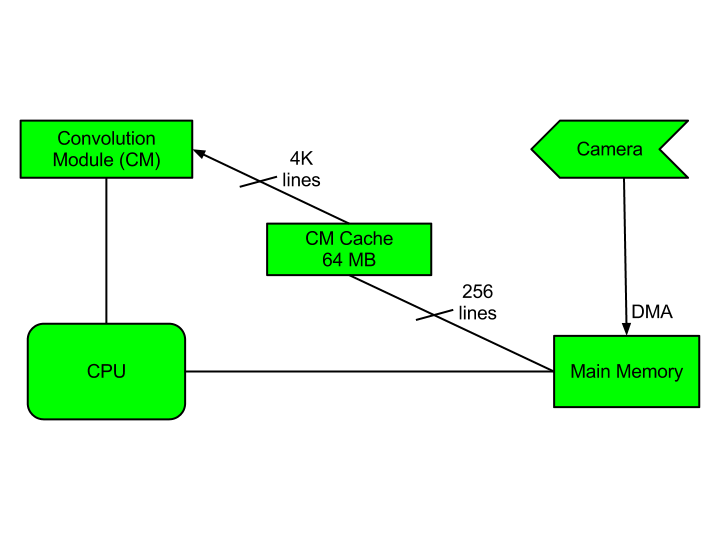
\includegraphics[width=90mm]{architecture.png}%
\captionof{figure}{}\label{fig:architecture}%
\end{center}

As input, the system uses a grayscale image stream of a camera at a fixed 512 x 512 pixel resolution at any standard frame rate (24, 30, 60 FPS). The camera feed is given DMA access to a fixed region of main memory. This will allow our dedicated cache to easily prefetch images as they arrive. On every hit, the CM cache will prefetch the next set of image data. This ensures a constant flow of data into the CM and ideally eliminates stall cycles caused by cache misses.  

During execution of the SIFT algorithm, our new ISA-level instruction will call the Convolution Module (CM) to begin convolving the image stream. Our implementation uses a fixed-size Gaussian kernel to speed up processing.  The design we developed  allows the CM to deal exclusively with the CM Cache at very high speed. Every cache hit will result in the next image being loaded into the CM module. Once there, every row in the image is convolved in parallel, granting us a massive speedup as discussed later.

%\begin{figure}[ht!]
%\centering
%\setlength\fboxsep{0pt}
%\setlength\fboxrule{0.5pt}
%\fbox{
%\includegraphics[width=90mm]{run1_max_error.png}
%}
%\caption{Plot of max of errors for Run 1, min/max revisited.}
%\label{fig:Run1_max_errors}
%\end{figure}

\subsection{Cache design}
\subsubsection{Organization}
Organization
The goal of the special convolution cache is to constantly feed the Convolution Module (CM) with data. We are not concerned with monetary cost or the transistor count of this hardware. We want the CM to execute a single row pass of convolution per call of the CONV instruction. Since our source images are 512x512, we need to give the CM module a cache line that is 512 words, with each word being 8 bits. To accomplish this, the interface to the cash from the CM has to be a 512 word wide bus. To reduce the hit time on the cache, we will use a direct mapped cache. The cache will use virtual addresses to once again keep hit time as low as possible. To avoid capacity misses, we need to use a cache that is at least big enough to keep an entire working set for an image in the cache. To avoid cold start misses, the cache will prefetch data from memory over a dedicated 8 word bus.

Since our application creates 3 octaves with 3 levels per octave per image, the total amount of memory used by one image will be 32x512x512 or 64 MB. This stems from the fact that we convolve an image across the rows, store that result, and then convolve the output of the row wise computation and store its output in the original image. This saves us a 512x512 chunk of memory per convolution.

Storing the convolution set of a single image in the cache is not enough because we want to keep the CM unit busy convolving images that are coming from the camera. Since a single image working set takes up so many resources, we can only store a few working sets in cache. Without simulation, it is impossible to figure out the optimal number. We choose to store only four working sets, making the total size of the cache 512 MB. This will enable us to do convolutions and other computations on one image while we prefetch the next images to be convolved.

{\bf Possibly add a pretty picture of cache here}

For the convolution results to be usable by the rest of the algorithm, the convolution cache has to be accessible by the regular CPU. To simplify the design, the convolution data's virtual addresses will be fixed. When the application code needs to access the convolution data to do calculations, a normal memory access will occur through a load instruction. Our convolution cache will be connected to the same bus as the level 1 cache and will service the load instructions that use the special virtual address range reserved for convolution data. This necessitates that our cache can handle two read requests in the same cycle and that supporting this does not affect hit time. We assume that the level 1 cache can ignore requests for this special address range and that this does not affect hit time on the level 1 cache.

\subsubsection{Performance}
With this cache organization, we expect the following performance. Due to prefetching and large capacity, we will have a hit rate from the CM close to 100\%. We assume that our system would be turned on once and expected to operate indefinitely, so initially the miss rate would be really high but quickly converge as the system operates. The hit rate from the CPU should also be close to 100\% for the same reasons. Thus, a single convolution can be performed in (3*512)*2 CPU cycles. (Load + execute + store ) Since a single image requires 16 convolutions, the total number of cycles to process an image would be 49152. Since our interface to main memory is 8 words wide, it will take 64*512  = 32768 cycles to prefetch the next image to be convolved. This is less than the time it takes to convolve an image. We assume that while one image is being convolved and another is being fetched from memory, the application can work on the intermediate results and that there is never a stall in the Convolution Module. This is why we chose to store four working sets in the cache instead of just one or two.
